\documentclass{article}
\usepackage[utf8]{inputenc}
\textheight = 25cm 
\textwidth = 15cm
\topmargin = -2.5cm 
\oddsidemargin = 1.5cm
\usepackage{hyperref}
\hypersetup{
    colorlinks=true,
    linkcolor=blue,
    filecolor=blue,
    citecolor = black,      
    urlcolor=cyan,
    }

\usepackage{float}
\usepackage{graphicx}

\usepackage{amsmath}
\usepackage{amsfonts}
\usepackage{mathtools, xparse}
\usepackage[shortlabels]{enumitem}
\usepackage[most]{tcolorbox}

\title{Tarea 2 Matemáticas Avanzadas de la Física}
\author{Cerritos Lira Carlos}
\date{2 de Marzo del 2020}

\begin{document}
\maketitle
Nota: código utilizado se encuentra en 
\url{https://github.com/carloscerlira/MAF/blob/master/Tarea_2/code.ipynb}
\section*{1.-}
Usar la transformada de Laplace para resolver las siguientes ecuaciones diferenciales
con condiciones iniciales y estudiar la gráfica de las soluciones.
\begin{enumerate}
    \item $y'' + 3y' + 2y = -5sin(t) + 5cos(t),\quad y_0 = 5,\quad y'_0 = 3$
    \item $y'' + y = 5h(t-\pi),\quad y_0=2,\quad y'_0 = 4$, donde $h(t)$ es la función de Heaviside.
    \item $y'' + 2y' + 2y = e^{-t} + 5\delta (t-2),\quad y_0 = 0,\quad y'_0=1$, donde $\delta(t)$ es la delta de Dirac.
    \item $ y'' + 8y' + 15y = 
    \begin{cases*}
        35e^{2t}, & si $0<t<2$ \\
        0,& caso contrario
    \end{cases*},\quad y_0=3, \quad y'_0=-8 $

\end{enumerate}
\begin{tcolorbox}
    \subsubsection*{Caso General}
    En el caso general se tiene:
    \begin{align*}
        Ay'' + By' + Cy &= f(t)\\
        A(p^2Y - py_0 - y_0') + B(pY - y_0) + CY &= F \\
        Y(Ap^2 + Bp + C) - (Ay_0p + Ay_0' + By_0) &= F \\
        Y &= \frac{1}{A(p+a)(p+b)}(F + Ay_0p + Ay_0' + By_0) \\
        Y &= \frac{1}{A}H(F + G) = \frac{1}{A} (Y_1 + Y_2) 
    \end{align*} 
    Resolvamos $Y_1 = HF$ \\ 
    En este caso tenemos $y_1 = f*h$, donde 
    \begin{align*}
        h(t) &= \frac{e^{-at} - e^{-bt}}{b-a},\quad a \neq b \\ 
        h(t) &= te^{-at},\quad a=b
    \end{align*}
    Resolvamos $Y_2 = HG$. \\
    En este caso tenemos $y_2 = g*h$, donde 
    \begin{align*}
        g(t) &= Ay_0\delta'(t) + (Ay_0' + By_0)\delta(t)
    \end{align*}
    calculando la convolución obtenemos:
    \begin{align*}
        g*h &=Ay_0 \delta'*h + (Ay_0' + By_0) \delta*h \\
        g*h &=Ay_0h' + (Ay_0' + By_0)h
    \end{align*}
    entonces la solución es $y = \frac{1}{A} (y_1 + y_2)$
\end{tcolorbox}
\begin{tcolorbox}
    \subsubsection*{1)}
    Hacemos cuentas para encontrar los parametros del caso general:
    \begin{align*}
        Ap^2 + Bp + C 
        &= p^2 + 3p + 2 \\
        &= (p+1)(p+2) 
    \end{align*}
    se tiene entonces:
    \begin{align*}
        A, B, C &= 1, 2, 3 \\ 
        a, b &= 1, 2 \\
        y_0, y_0' &= 5, 3
    \end{align*}
    entonces nuestra solución es:
    \[ y = f*h + g*h \]
    resolviendo numéricamente $f*h$ encontramos la gráfica de $y$:
    \begin{figure}[H]
        \centering
        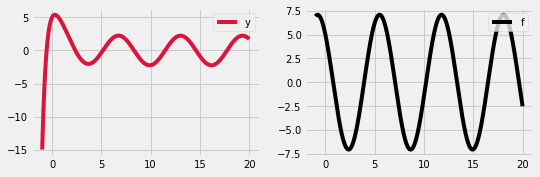
\includegraphics[scale=0.7]{images/p1_1.png}
    \end{figure}

    \subsubsection*{2)}
    Hacemos cuentas para encontrar los parametros del caso general:
    \begin{align*}
        Ay^2 + By + C 
        &= y^2 + y \\
        &= (y+1)(y+0)
    \end{align*}
    se tiene entonces:
    \begin{align*}
        A, B, C &= 1,1,0 \\ 
        a,b &= 1,0 \\
        y_0, y_0' &= 2, 4
    \end{align*}
    entonces nuestra solución es:
    \[ y = f*h + g*h \]
    resolviendo numéricamente $f*h$ encontramos la gráfica de $y$:
    \begin{figure}[H]
        \centering
        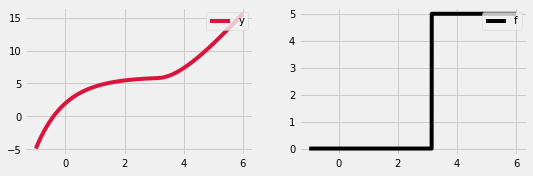
\includegraphics[scale=0.7]{images/p1_2.png}
    \end{figure}
\end{tcolorbox}
\begin{tcolorbox}
    \subsubsection*{3)}
    Hacemos cuentas para encontrar los parametros del caso general:
    \begin{align*}
        Ay^2 + By + C 
        &= y^2 + 2y + 2 \\
        &= (y+1+i)(y+1-i)
    \end{align*}
    se tiene entonces:
    \begin{align*}
        A, B, C &= 1, 2, 2 \\ 
        a,b &= 1+i, 1-i \\  
        y_0, y_0' &= 0,1
    \end{align*}    
    entonces nuestra solución es:
    \[ y = f*h + g*h \]
    resolviendo numéricamente $f*h$ encontramos la gráfica de $y$:
    \begin{figure}[H]
        \centering
        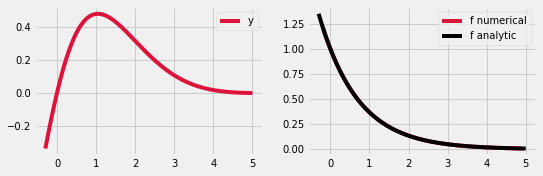
\includegraphics[scale=0.7]{images/p1_3.png}
    \end{figure}

    \subsubsection*{4)}
    Hacemos cuentas para encontrar los parametros del caso general:
    \begin{align*}
        Ay^2 + By + C 
        &= y^2 + 8y + 15 \\
        &= (y+5)(y+3)
    \end{align*}
    se tiene entonces:
    \begin{align*}
        A, B, C &= 1,8,15 \\
        a,b &= 5,3 \\ 
        y_0, y_0' &= 3,-8
    \end{align*}
    entonces nuestra solución es:
    \[ y = f*h + g*h \]
    resolviendo numéricamente $f*h$ encontramos la gráfica de $y$:
    \begin{figure}[H]
        \centering
        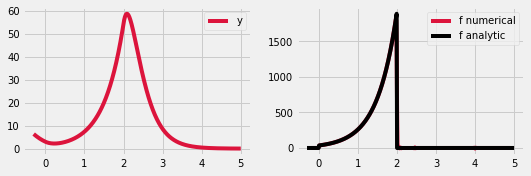
\includegraphics[scale=0.7]{images/p1_4.png}
    \end{figure}

\end{tcolorbox}

\section*{2.-}
Se define el siguiente conjunto de funciones (llamado lorentziano):
\[
f_\epsilon(t)=\frac{1}{\pi}\frac{\epsilon}{t^2+\epsilon^2}, t\in\mathbb{R}, 
\epsilon \ge>0.
\]
\begin{enumerate}[a)]
    \item Argumentar que $\lim_{\epsilon\to0^+}f_\epsilon(t)=\delta(t)$, 
    donde $\delta(t)$ es la delta de Dirac. 
    \item A partir de $f_\epsilon(t)$ obtener un conjunto de funciones que aproximen a la función de Heaviside $h(t)$, a $\delta'(t)$ y 
    a $\delta''(t)$ y estudiar las correspondientes gráficas. 
\end{enumerate}
\begin{tcolorbox}

\end{tcolorbox}

\section*{3.-} 
En los siguientes cuatro 4 apartados, a partir de las soluciones
de la ecuación homogénea dadas, obtener una solución particular 
de la ecuación no homogénea usando funciones de Green.
\begin{enumerate}[a)]
    \item $y''-y=sech(x)$, con $sinh(x), cosh(x)$ soluciones de la homogénea.
    \item $x^2y''-2xy'+2y=xlog(x)$, con $x, x^2$ soluciones de la homogénea.
    \item $y''-2cosec^2(x)y=sin^2(x)$, con $cotg(x), 1-xcotg(x)$ soluciones de la homogénea.
    \item $(x^2+1)y''-2xy'+2y=(x^2+1)^2$, con $x, 1-x^2$ soluciones de la homogénea.
\end{enumerate}
\begin{tcolorbox}
    \subsubsection*{Caso General}
    En el caso general tenemos la ecuación:
    \begin{align*}
        y''(x) + p(x)y'(x) + q(x)y(x) &= f(x), \quad y(a) = y(b) = 0
    \end{align*}
    la solucuión esta dada por:
    \begin{align*}
        y(x) &= \int_{a}^b G(x,x')f(x')dx'
    \end{align*}
    donde $G$ esta definida por:
    \begin{align*}
        G(x,x') &=
        \begin{cases*}
            A(x')y_1(x), & si $0<x<x'<b$ \\
            B(x')y_2(x),& si $a<x'<x<b$
        \end{cases*}  
    \end{align*}
    donde:
    \begin{align*}
        A &= \frac{y_2}{w} 
        \quad B = \frac{y_1}{w} \\ 
        w &= y_1y_2'-y_1'y_2
    \end{align*}
    con $y_1,y_2$ soluciones de la ecuación homogénea 
    que satisfacen $y_1(a) = y_2(b) = 0$. \\ \\
    Observamos entonces que la solción esta expresada por:
    \begin{align*}
        y &= y_2\int_{a}^x Bf dx' + y_1\int_{x}^b Afdx' 
    \end{align*}
    es importante notar que si $y_1, y_2$ son soluciones de la ecación homogénea
    entonces 
    \[ y = y_1 \pm y_2 \] 
    es solución de la ecuación homogénea.
    
    
\end{tcolorbox}
\begin{tcolorbox}
    \subsubsection*{1)}
    Hacemos cuentas para obtener los parametros del caso general:
    \begin{align*}
        f&= sech \\
        a&=0 &&b=\frac{1}{2}\pi \\
        p&=0 &&q=-1 \\
        y_1 &= sinh  &&y_2= cosh(x-b)-1 \\
        y_1' &= cosh &&y_2'=sinh 
    \end{align*}
    de donde obtenemos $y$ resolviendo la integral numéricamente:
    \begin{figure}[H]
        \centering
        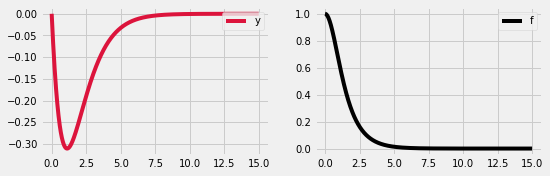
\includegraphics[scale=0.7]{images/p3_1.png}
    \end{figure}

    \subsubsection*{2)}
    Hacemos cuentas para obtener los parametros del caso general:
    \begin{align*}
        f&= \frac{logx}{x} \\
        a&=0 &&b=1 \\
        p&=\frac{-2}{x} &&q= \frac{2}{x^2} \\
        y_1 &= x^2  &&y_2= x^2-x \\
        y_1' &= 2x &&y_2'= 2x-1 
    \end{align*}
    de donde obtenemos $y$ resolviendo la integral numéricamente:
    \begin{figure}[H]
        \centering
        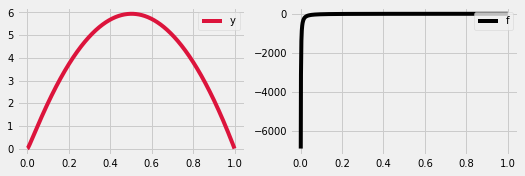
\includegraphics[scale=0.7]{images/p3_2.png}
    \end{figure}
\end{tcolorbox}
\begin{tcolorbox}
    \subsubsection*{3)}
    Hacemos cuentas para obtener los parametros del caso general:
    \begin{align*}
        f&= sin^2x \\
        a&=0 &&b=\frac{1}{2}\pi \\
        p&=0 &&q= -2cscx^2 \\
        y_1 &= 1-xcotx  &&y_2= cotx \\
        y_1' &= -cotx + xcsc^2x  &&y_2'= -csc^2x 
    \end{align*}
    de donde obtenemos $y$ resolviendo la integral numéricamente:
    \begin{figure}[H]
        \centering
        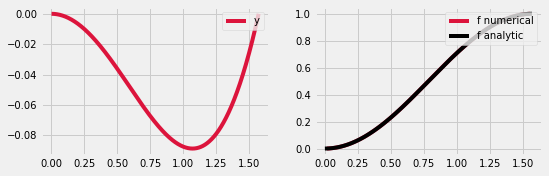
\includegraphics[scale=0.7]{images/p3_3.png}
    \end{figure}

    \subsubsection*{4)}
    Hacemos cuentas para obtener los parametros del caso general:
    \begin{align*}
        f&= 1 \\
        a &=0 &&b=1 \\
        p &=\frac{-2x}{x^2+1} &&q= \frac{2}{x^2+1} \\
        y_1 &=x  &&y_2= 1-x^2 \\
        y_1' &=1 &&y_2'= -2x  
    \end{align*}
    de donde obtenemos $y$ resolviendo la integral numéricamente:
    \begin{figure}[H]
        \centering
        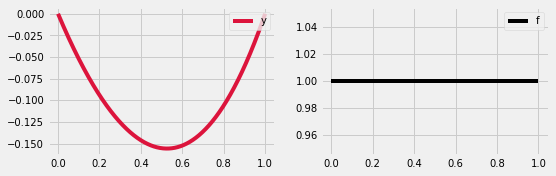
\includegraphics[scale=0.7]{images/p3_4.png}
    \end{figure}

\end{tcolorbox}



\section*{4.-}
Resolver las siguientes ecuaciones en derivadas parciales con 
condiciones iniciales usando el método de separación de variables:
\begin{enumerate}[a)]
    \item $\frac{\partial^2u}{\partial x^2}+\frac{\partial^2u}{\partial y^2}+\frac{\partial^2u}{\partial z^2}=0$ en $\Omega=\{(x,y,z)\in \mathbb{R}^3: 0<x,y<c, 0<z<L\}$ con $u(x,y,z)$ anulándose en todos los lados del parlelepípedo excepto en $z=L$ donde $u(x,y,L)=V$.
    \item $-\left(\frac{\partial^2u}{\partial x^2}+\frac{\partial^2u}{\partial y^2}+\frac{\partial^2u}{\partial z^2}\right)=Eu$ en $\Omega=\{(x,y,z)\in\mathbb{R}^3: 0<x<a,0<y<b, 0<z<c\}$
    con $u(x,y,z)$ anulándose en todos los lados del paralelepípedo. 
\end{enumerate}
\begin{tcolorbox}
    
\end{tcolorbox}
\section*{Bibliografía}
\begin{itemize}
    \item \textit{Mathematical Methods in the Physical Sciences}. Boas, Mary. Tercera Edición. Lehigh Press. 2006. Cap.
\end{itemize}

\end{document}